\documentclass[12pt,a4paper]{article}
\usepackage[spanish,es-tabla]{babel}
\usepackage{float}							% Insertar figuras
\usepackage{subfig}

\usepackage[utf8]{inputenc} % Escribir con acentos, ~n...
\usepackage{eurosym} % s´ımbolo del euro
\newcommand{\horrule}[1]{\rule{\linewidth}{#1}} % Create horizontal rule command with 1 argument of height
\usepackage{listings}             % Incluye el paquete listing
\usepackage[cache=false]{minted}
\usepackage{graphics,graphicx, float} %para incluir imágenes y colocarlas
\usepackage{hyperref}
\hypersetup{
	colorlinks,
	citecolor=black,
	filecolor=black,
	linkcolor=black,
	urlcolor=black
}
\usepackage{multirow}
\usepackage{array}
\usepackage{diagbox}
\usepackage{listings}

\lstset{language=Java,
	keywordstyle=\color{RoyalBlue},
	basicstyle=\scriptsize\ttfamily,
	commentstyle=\ttfamily\itshape\color{gray},
	stringstyle=\ttfamily,
	showstringspaces=false,
	breaklines=true,
	frameround=ffff,
	frame=single,
	rulecolor=\color{black}}
\title{
\normalfont \normalsize 
\textsc{{\bf Servidores web de altas prestaciones (2019-2020)} \\ Grado en Ingeniería Informática \\ Universidad de Granada} \\ [25pt] % Your university, school and/or department name(s)
\horrule{0.5pt} \\[0.4cm] % Thin top horizontal rule
\huge Práctica 1 \\ % The assignment title
\horrule{2pt} \\[0.5cm] % Thick bottom horizontal rule

\includegraphics{images/logo.png}	
}

\author{Antonio Jesús Heredia Castillo} % Nombre y apellidos

\date{\normalsize\today} % Incluye la fecha actual

%----------------------------------------------------------------------------------------
% DOCUMENTO
%----------------------------------------------------------------------------------------

\begin{document}

\maketitle % Muestra el Título
\newpage %inserta un salto de página
\tableofcontents % para generar el índice de contenidos
\newpage
\section{Configuración de Netplan}
Como los pasos de instalación de las maquinas virtuales y de los servicios correspondientes vienen explicados en el guión de practicas, paso directamente a explicar la configuración usada en el netplan. 
\begin{figure}[H]
	\centering
	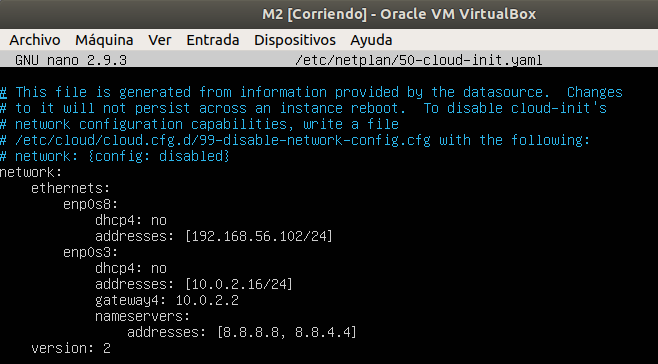
\includegraphics[width=1\linewidth]{images/netplanm2}
	\caption{Netplan de la maquina M2.}
	\label{fig:netplanm2}
\end{figure}
En la Figura \ref{fig:netplanm2} podemos ver la configuración de la maquina M2. Que paso a explicar. En el fichero podemos ver como configuramos dos interfaces de red. Una llamada \textbf{enp0s8} y otra llamada \textbf{enp0s3}. La interfaz \textbf{enp0s8} corresponde al "solo-anfitrión" del Virtual Box, debido a esto esa interfaz no necesita ni puerta de enlace ni servidores DNS. Solo especificamos la dirección estática que tendrá para tener conexión \textbf{enp0s3} es la red NAT, que es la que nos da salida a internet desde nuestra maquina virtual. Por ello ha esta le debemos poner la puerta de enlace y la dirección de los servidores DNS.  

Para evitar escribir el documento entero de nuevo decidí copiarlo mediante SCP y pasarlo de M2 a M1. Para ello realicé el comando que se puede ver en la Figura \ref{fig:scp}. 

\begin{figure}[H]
	\centering
	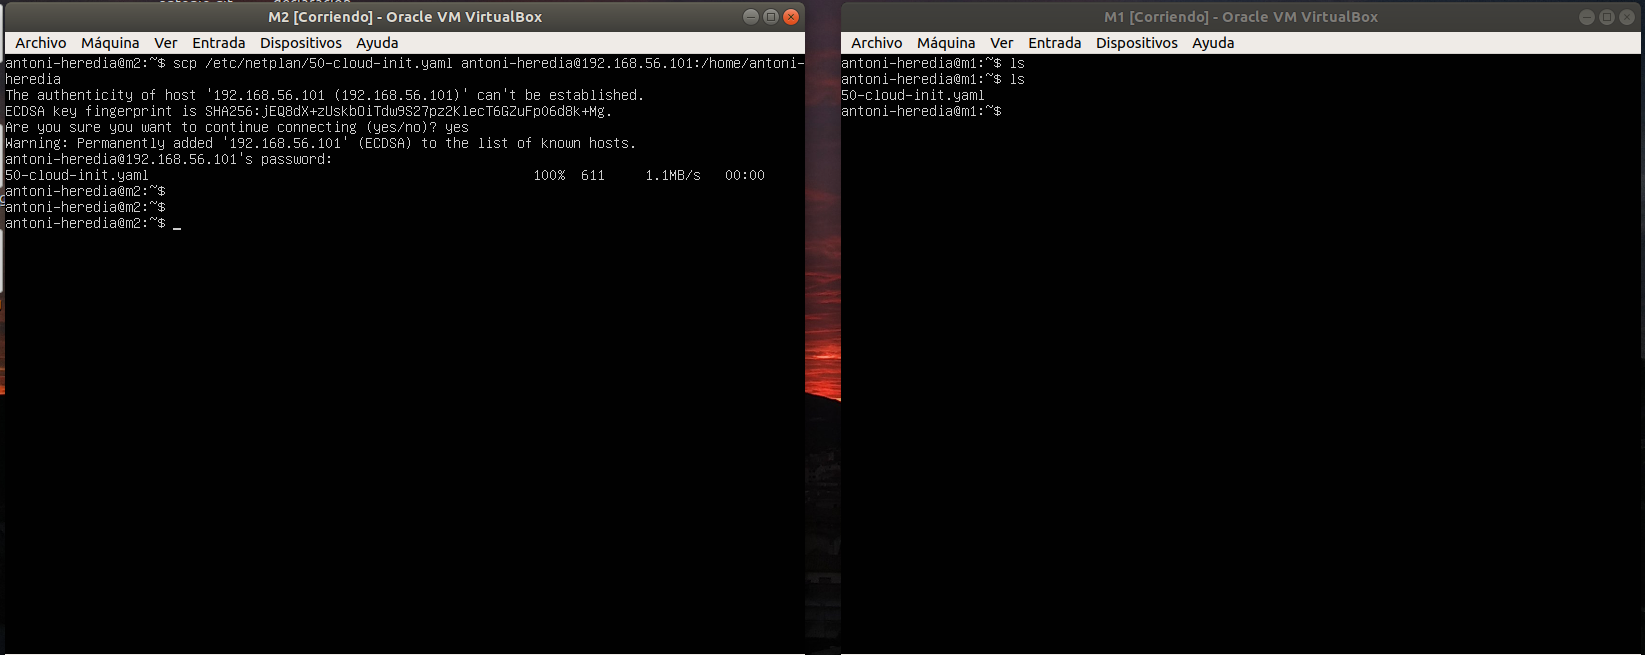
\includegraphics[width=1\linewidth]{images/scp}
	\caption{Copia del netplan a la maquina M1}
	\label{fig:scp}
\end{figure}
Finalmente tendremos la configuración que podemos ver en la Figura \ref{fig:netplanm1} en la maquina M1. 
\begin{figure}[H]
	\centering
	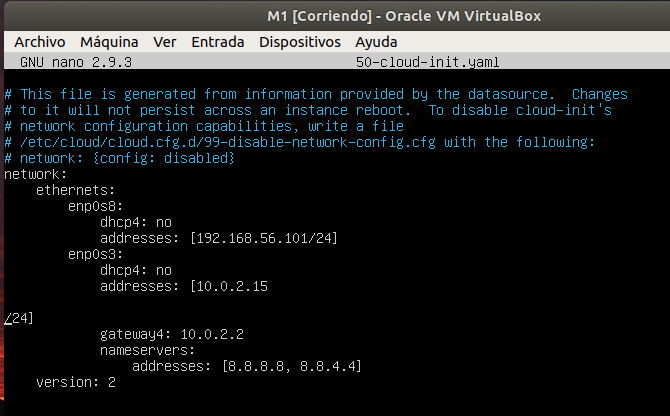
\includegraphics[width=1\linewidth]{images/netplanm1}
	\caption{Netplan de la maquina M1.}
	\label{fig:netplanm1}
\end{figure}
\section{Comprobación conexion a internet}
Para ver si la configuración del netplan es correcta realizaremos un ping a una dirección de internet (por ejempolo google.com) en ambas maquinas. En al Figura \ref{f:internetm1} podemos que ambas maquinas pueden hacer ping. 
\begin{figure}[H]
	\centering
	\subfloat[Maquina M1]{
		\label{f:internet1}
		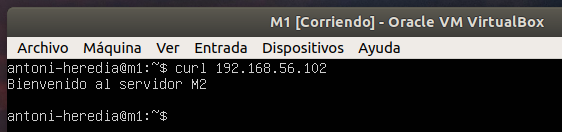
\includegraphics[width=0.5\textwidth]{images/internet1.png}}
	\subfloat[Maquina M2]{
		\label{f:modTablaB}
		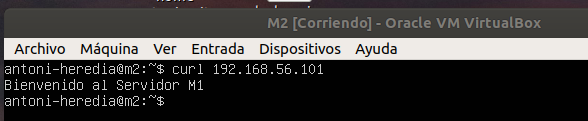
\includegraphics[width=0.5\textwidth]{images/internet2.png}}
	\caption{Comprobación de salida a internet de ambas maquinas.}
	
	\label{f:internetm1}
\end{figure}
\section{Comprobación conexión entre maquinas}
Para comprobar si las maquinas estan conectadas entresi y ademas tienen el servidor Apache bien configurado y funcionando usaremos la herramienta \textbf{curl}. Con ella podemos hacer una petición web que nos devolverá en texto plano el contenido de la web. Ambas maquinas están ofreciendo en el puerto 80 en el index un fichero en texto plano con el contenido que se especifica en el guión de practicas. En la Figura \ref{f:maquinas} podemos ver el resultado de realizar curl de una maquina a la otra. 
\begin{figure}[H]
	\centering
	\subfloat[Maquina M1]{
		\label{f:con1}
		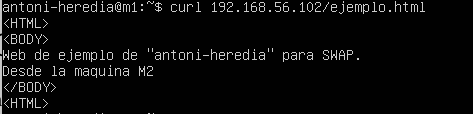
\includegraphics[width=0.5\textwidth]{images/curl2.png}}
	\subfloat[Maquina M2]{
		\label{f:con2}
		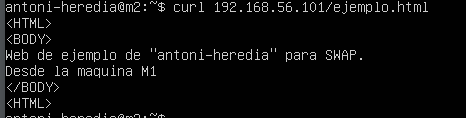
\includegraphics[width=0.5\textwidth]{images/curl1.png}}
	\caption{Comprobación de apache en ambas.}
	
	\label{f:maquinas}
\end{figure}

Para comprobar si el servidor ssh esta bien configurado en ambas maquinas bastara con hacer las comprobaciones que podemos ver en la Figura \ref{label}. Como tenemos el mismo usuario en ambas maquinas no hará falta especificarlo, solo usar la contraseña. 
\begin{figure}[H]
	\centering
	\subfloat[Maquina M1]{
		\label{f:ssh1}
		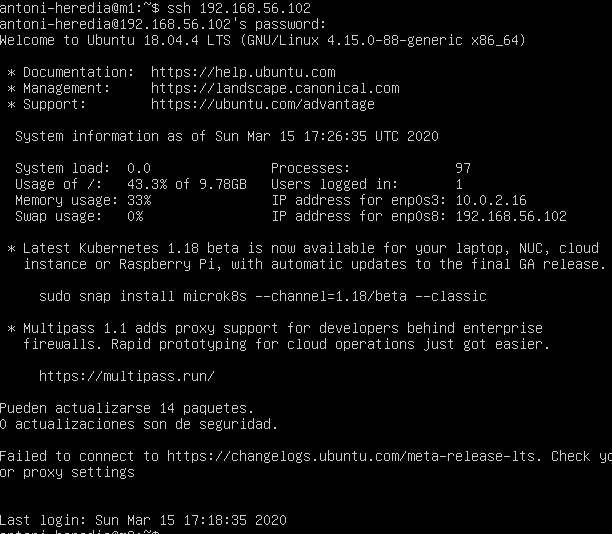
\includegraphics[width=0.5\textwidth]{images/ssh1.png}}
	\subfloat[Maquina M2]{
		\label{f:ssh2}
		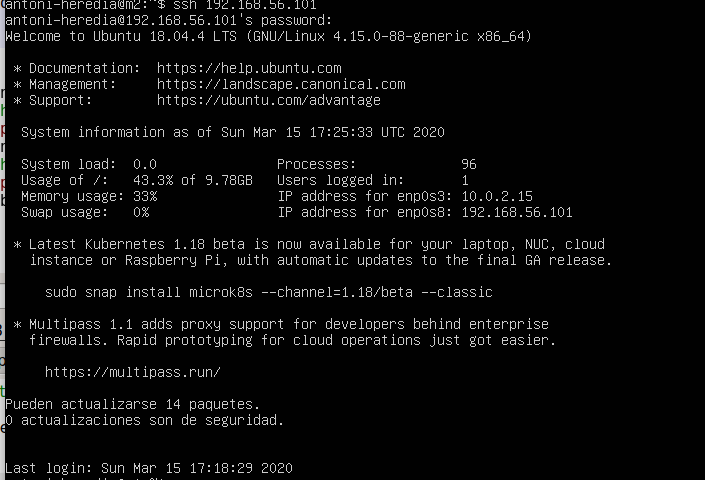
\includegraphics[width=0.5\textwidth]{images/ssh2.png}}
	\caption{Comprobación de conexión entre ambas maquinas.}
	
	\label{f:ssh}
\end{figure}
\end{document}
	